\documentclass[11pt,preprint, authoryear]{elsarticle}

\usepackage{lmodern}
%%%% My spacing
\usepackage{setspace}
\setstretch{1.2}
\DeclareMathSizes{12}{14}{10}{10}

% Wrap around which gives all figures included the [H] command, or places it "here". This can be tedious to code in Rmarkdown.
\usepackage{float}
\let\origfigure\figure
\let\endorigfigure\endfigure
\renewenvironment{figure}[1][2] {
    \expandafter\origfigure\expandafter[H]
} {
    \endorigfigure
}

\let\origtable\table
\let\endorigtable\endtable
\renewenvironment{table}[1][2] {
    \expandafter\origtable\expandafter[H]
} {
    \endorigtable
}


\usepackage{ifxetex,ifluatex}
\usepackage{fixltx2e} % provides \textsubscript
\ifnum 0\ifxetex 1\fi\ifluatex 1\fi=0 % if pdftex
  \usepackage[T1]{fontenc}
  \usepackage[utf8]{inputenc}
\else % if luatex or xelatex
  \ifxetex
    \usepackage{mathspec}
    \usepackage{xltxtra,xunicode}
  \else
    \usepackage{fontspec}
  \fi
  \defaultfontfeatures{Mapping=tex-text,Scale=MatchLowercase}
  \newcommand{\euro}{€}
\fi

\usepackage{amssymb, amsmath, amsthm, amsfonts}

\def\bibsection{\section*{References}} %%% Make "References" appear before bibliography


\usepackage[round]{natbib}

\usepackage{longtable}
\usepackage[margin=2.3cm,bottom=2cm,top=2.5cm, includefoot]{geometry}
\usepackage{fancyhdr}
\usepackage[bottom, hang, flushmargin]{footmisc}
\usepackage{graphicx}
\numberwithin{equation}{section}
\numberwithin{figure}{section}
\numberwithin{table}{section}
\setlength{\parindent}{0cm}
\setlength{\parskip}{1.3ex plus 0.5ex minus 0.3ex}
\usepackage{textcomp}
\renewcommand{\headrulewidth}{0.2pt}
\renewcommand{\footrulewidth}{0.3pt}

\usepackage{array}
\newcolumntype{x}[1]{>{\centering\arraybackslash\hspace{0pt}}p{#1}}

%%%%  Remove the "preprint submitted to" part. Don't worry about this either, it just looks better without it:
\makeatletter
\def\ps@pprintTitle{%
  \let\@oddhead\@empty
  \let\@evenhead\@empty
  \let\@oddfoot\@empty
  \let\@evenfoot\@oddfoot
}
\makeatother

 \def\tightlist{} % This allows for subbullets!

\usepackage{hyperref}
\hypersetup{breaklinks=true,
            bookmarks=true,
            colorlinks=true,
            citecolor=blue,
            urlcolor=blue,
            linkcolor=blue,
            pdfborder={0 0 0}}


% The following packages allow huxtable to work:
\usepackage{siunitx}
\usepackage{multirow}
\usepackage{hhline}
\usepackage{calc}
\usepackage{tabularx}
\usepackage{booktabs}
\usepackage{caption}


\newenvironment{columns}[1][]{}{}

\newenvironment{column}[1]{\begin{minipage}{#1}\ignorespaces}{%
\end{minipage}
\ifhmode\unskip\fi
\aftergroup\useignorespacesandallpars}

\def\useignorespacesandallpars#1\ignorespaces\fi{%
#1\fi\ignorespacesandallpars}

\makeatletter
\def\ignorespacesandallpars{%
  \@ifnextchar\par
    {\expandafter\ignorespacesandallpars\@gobble}%
    {}%
}
\makeatother

\newenvironment{CSLReferences}[2]{%
}

\urlstyle{same}  % don't use monospace font for urls
\setlength{\parindent}{0pt}
\setlength{\parskip}{6pt plus 2pt minus 1pt}
\setlength{\emergencystretch}{3em}  % prevent overfull lines
\setcounter{secnumdepth}{5}

%%% Use protect on footnotes to avoid problems with footnotes in titles
\let\rmarkdownfootnote\footnote%
\def\footnote{\protect\rmarkdownfootnote}
\IfFileExists{upquote.sty}{\usepackage{upquote}}{}

%%% Include extra packages specified by user

%%% Hard setting column skips for reports - this ensures greater consistency and control over the length settings in the document.
%% page layout
%% paragraphs
\setlength{\baselineskip}{12pt plus 0pt minus 0pt}
\setlength{\parskip}{12pt plus 0pt minus 0pt}
\setlength{\parindent}{0pt plus 0pt minus 0pt}
%% floats
\setlength{\floatsep}{12pt plus 0 pt minus 0pt}
\setlength{\textfloatsep}{20pt plus 0pt minus 0pt}
\setlength{\intextsep}{14pt plus 0pt minus 0pt}
\setlength{\dbltextfloatsep}{20pt plus 0pt minus 0pt}
\setlength{\dblfloatsep}{14pt plus 0pt minus 0pt}
%% maths
\setlength{\abovedisplayskip}{12pt plus 0pt minus 0pt}
\setlength{\belowdisplayskip}{12pt plus 0pt minus 0pt}
%% lists
\setlength{\topsep}{10pt plus 0pt minus 0pt}
\setlength{\partopsep}{3pt plus 0pt minus 0pt}
\setlength{\itemsep}{5pt plus 0pt minus 0pt}
\setlength{\labelsep}{8mm plus 0mm minus 0mm}
\setlength{\parsep}{\the\parskip}
\setlength{\listparindent}{\the\parindent}
%% verbatim
\setlength{\fboxsep}{5pt plus 0pt minus 0pt}



\begin{document}



\begin{frontmatter}  %

\title{Question 1: Something here}

% Set to FALSE if wanting to remove title (for submission)




\author[Add1]{Hendri van Zyl}
\ead{17640296@sun.ac.za}





\address[Add1]{Stellenbosch, South Africa}


\begin{abstract}
\small{
Compare SWIX and ALSI methodologies by looking at different sector
exposures and stock concentration over time.
}
\end{abstract}

\vspace{1cm}


\begin{keyword}
\footnotesize{
Portfolio Construction\sep SWIX vs ALSI \sep JSE \\
\vspace{0.3cm}
}
\end{keyword}



\vspace{0.5cm}

\end{frontmatter}

\setcounter{footnote}{0}



%________________________
% Header and Footers
%%%%%%%%%%%%%%%%%%%%%%%%%%%%%%%%%
\pagestyle{fancy}
\chead{}
\rhead{}
\lfoot{}
\rfoot{\footnotesize Page \thepage}
\lhead{}
%\rfoot{\footnotesize Page \thepage } % "e.g. Page 2"
\cfoot{}

%\setlength\headheight{30pt}
%%%%%%%%%%%%%%%%%%%%%%%%%%%%%%%%%
%________________________

\headsep 35pt % So that header does not go over title




\hypertarget{introduction}{%
\section*{Introduction}\label{introduction}}
\addcontentsline{toc}{section}{Introduction}

The SWIX (Shareholder Weighted Indices) and ALSI (All Share Index) are
both methodologies used in the South African financial markets for index
construction, but they differ in their approaches and compositions.

\hypertarget{swix-shareholder-weighted-indices}{%
\subsubsection*{SWIX (Shareholder Weighted
Indices):}\label{swix-shareholder-weighted-indices}}
\addcontentsline{toc}{subsubsection}{SWIX (Shareholder Weighted
Indices):}

\emph{The SWIX methodology adjusts the market capitalization of
companies based on the portion of shares that are available to local
investors. }It reduces the weighting of companies in the index that have
a large proportion of their shares held by foreign or strategic
investors, who are less likely to trade these shares actively.
\emph{This methodology is designed to provide a more accurate reflection
of the investable market for local investors, as it focuses on the
free-float shares that are actually available for trading in the
domestic market. }SWIX is considered to give a better indication of what
local investors are likely to experience in terms of market movements
and is often used by local fund managers for benchmarking.

\hypertarget{alsi-all-share-index}{%
\subsubsection*{ALSI (All Share Index):}\label{alsi-all-share-index}}
\addcontentsline{toc}{subsubsection}{ALSI (All Share Index):}

\emph{The ALSI represents the performance of the South African stock
market by including all listed companies on the Johannesburg Stock
Exchange (JSE). }It is a market capitalization-weighted index, meaning
that companies with a higher market cap have a larger influence on the
index's performance. \emph{The ALSI does not adjust for the shareholder
base, so it includes both domestic and foreign-held shares in its
calculation. }It provides a broad representation of the South African
stock market, making it a useful tool for understanding overall market
performance.

\hypertarget{compare-cumulative-returns-for-various-cap-sizes}{%
\subsection*{Compare cumulative returns for various cap
sizes}\label{compare-cumulative-returns-for-various-cap-sizes}}
\addcontentsline{toc}{subsection}{Compare cumulative returns for various
cap sizes}

\hypertarget{large-caps}{%
\subsubsection*{Large caps}\label{large-caps}}
\addcontentsline{toc}{subsubsection}{Large caps}

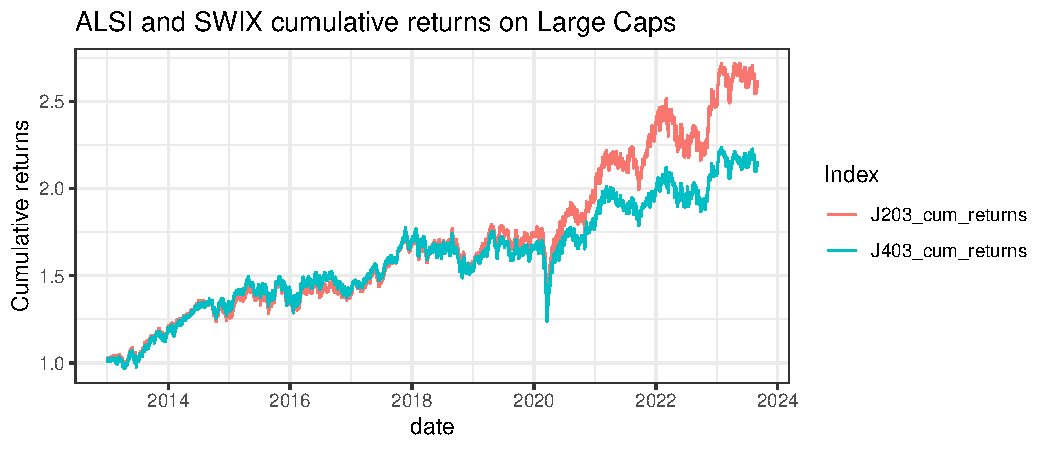
\includegraphics{Question3_files/figure-latex/unnamed-chunk-1-1.pdf}

The cumulative return series for the J203 or ALSI appears to outperform
the J403 or the SWIX method in the long run for large caps.

\hypertarget{medium-caps}{%
\subsubsection*{Medium Caps}\label{medium-caps}}
\addcontentsline{toc}{subsubsection}{Medium Caps}

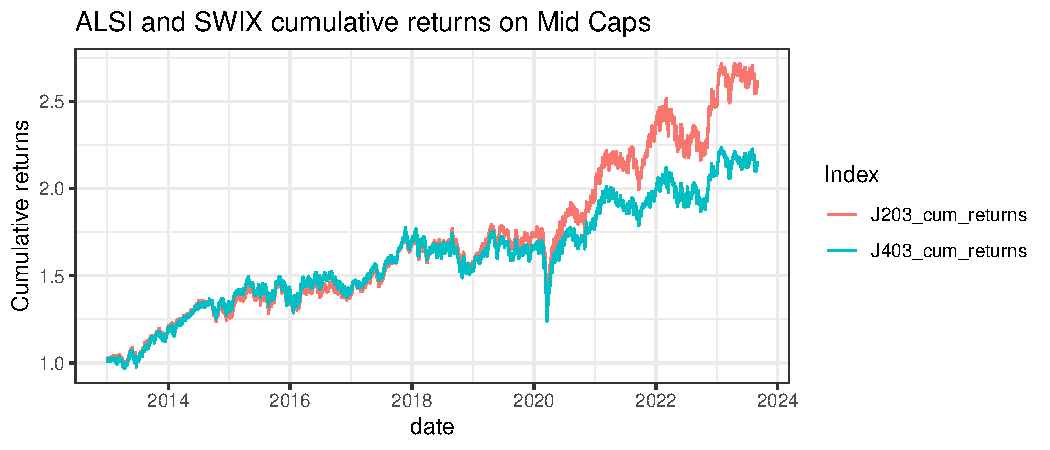
\includegraphics{Question3_files/figure-latex/unnamed-chunk-2-1.pdf}

\hypertarget{small-caps}{%
\subsubsection*{Small Caps}\label{small-caps}}
\addcontentsline{toc}{subsubsection}{Small Caps}

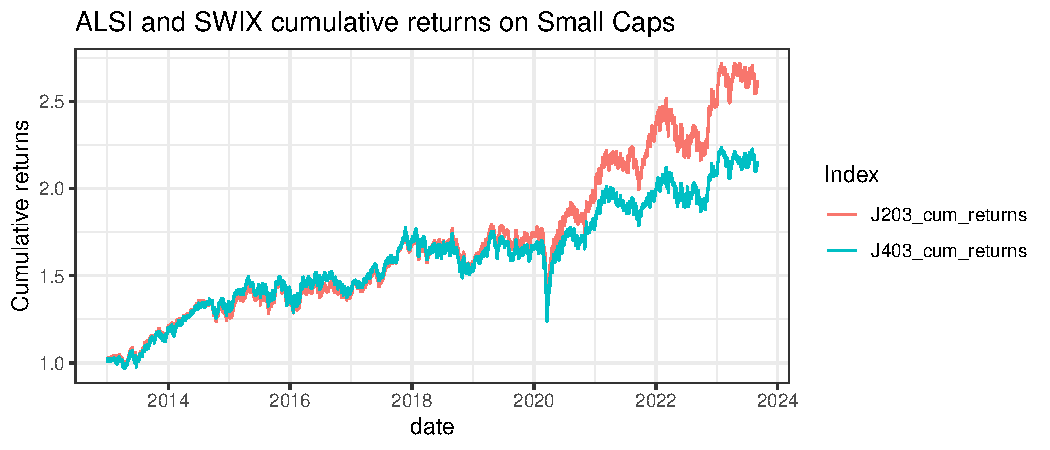
\includegraphics{Question3_files/figure-latex/unnamed-chunk-3-1.pdf}

All three identical. What a coincidence!

\hypertarget{compare-methods-by-cumulative-returns-per-sector}{%
\subsection*{Compare methods by cumulative returns per
sector}\label{compare-methods-by-cumulative-returns-per-sector}}
\addcontentsline{toc}{subsection}{Compare methods by cumulative returns
per sector}

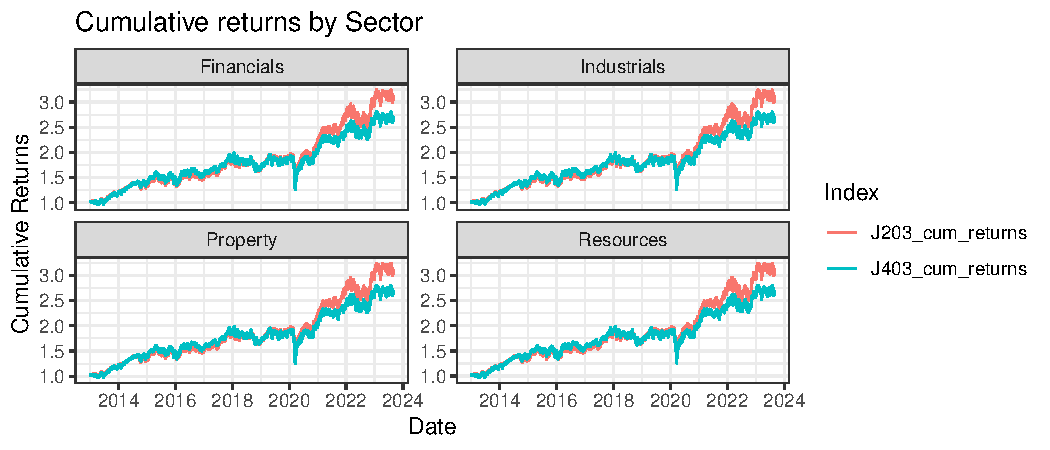
\includegraphics{Question3_files/figure-latex/unnamed-chunk-4-1.pdf}

Again identical. Amazing\ldots{}

\hypertarget{conclusion}{%
\section*{Conclusion}\label{conclusion}}
\addcontentsline{toc}{section}{Conclusion}

I'm sorry about this.

\bibliography{Tex/ref}





\end{document}
